\caulc
\begin{ex}%[1D6H2-2]%[TDMZZ19]%[Trần Văn Thiện, Nguyễn Sơn Thành]
	Cho $a = \log_2 3$ và $b = \log_2 7$. Giá trị $\log_4 63$ bằng
	\choice
	{$\dfrac{a + 2b}{2}$}
	{$a + 2b$}
	{\True $\dfrac{2a + b}{2}$}
	{$4a + 2b$}
	\loigiai{
		Ta có
		\begin{eqnarray*}
			\log_4 63&= & \log_{2^2} (3^2 \cdot 7)\\
			&= & \dfrac{1}{2} \log_2 (3^2 \cdot 7)
		\end{eqnarray*}
		Lại có $\dfrac{1}{2} \log_2 (3^2 \cdot 7) = \dfrac{1}{2} \big( \log_2 3^2 + \log_2 7 \big) = \dfrac{1}{2} \big( 2\log_2 3 + \log_2 7 \big)$.\\
		Thay $a = \log_2 3$ và $b = \log_2 7$ ta được $\log_4 63 = \dfrac{2a + b}{2}$.
	}
\end{ex}

\begin{ex}%[1D3H2-4]%[TDMZZ19]%[Trần Văn Thiện, Nguyễn Sơn Thành]
	Giá trị của $\lim\limits_{x \to +\infty} \dfrac{x + \sqrt{x^4 - 1}}{x\sqrt{x} + 2}$ bằng
	\choice
	{\True $+\infty$}
	{$0$}
	{$-\infty$}
	{$2$}
	\loigiai{
		Ta có $\lim\limits_{x \to +\infty} \dfrac{x + \sqrt{x^4 - 1}}{x\sqrt{x} + 2} = \lim\limits_{x \to +\infty} \dfrac{x^2\left(\dfrac{1}{x} + \sqrt{1 - \dfrac{1}{x^4}}\right)}{x\sqrt{x}\left(1 + \dfrac{2}{x\sqrt{x}}\right)} = \lim\limits_{x \to +\infty} \left( \sqrt{x} \cdot \dfrac{\dfrac{1}{x} + \sqrt{1 - \dfrac{1}{x^4}}}{1 + \dfrac{2}{x\sqrt{x}}} \right)$.\\
		Vì $\lim\limits_{x \to +\infty} \sqrt{x} = +\infty$ và $\lim\limits_{x \to +\infty} \dfrac{\dfrac{1}{x} + \sqrt{1 - \dfrac{1}{x^4}}}{1 + \dfrac{2}{x\sqrt{x}}} = \dfrac{0 + 1}{1 + 0} = 1 > 0$.\\
		Do đó $\lim\limits_{x \to +\infty} \dfrac{x + \sqrt{x^4 - 1}}{x\sqrt{x} + 2} = +\infty$.
	}
\end{ex}

\begin{ex}%[1D6H4-4]%[TDMZZ19]%[Trần Văn Thiện, Nguyễn Sơn Thành]
	Phương trình $9^{x^2 - 2} = 27^4$ có tập nghiệm là
	\choice
	{\True $\{\pm 2\sqrt{2}\}$}
	{$\{\pm 2\}$}
	{$\{\pm 4\}$}
	{$\{1; 4\}$}
	\loigiai{
		Ta có
		\begin{eqnarray*}
			& & 9^{x^2 - 2} = 27^4\\
			&\Leftrightarrow & \left(3^2\right)^{x^2 - 2} = \left(3^3\right)^4\\
			&\Leftrightarrow & 3^{2x^2 - 4} = 3^{12}\\
			& \Leftrightarrow& 2x^2 - 4 = 12\\
			&\Leftrightarrow & 2x^2 = 16\\
			&\Leftrightarrow & x^2 = 8 \\
			&\Leftrightarrow & x = \pm 2\sqrt{2}.
		\end{eqnarray*}
		Vậy tập nghiệm của phương trình là $S = \{\pm 2\sqrt{2}\}$.
	}
\end{ex}

\begin{ex}%[1H8H7-5]%[TDMZZ19]%[Trần Văn Thiện, Nguyễn Sơn Thành]
	Cho một hình hộp chữ nhật $ABCD. A'B'C'D'$ có kích thước các cạnh $AB = a$, $AD = 2a$, $AA' = 2a$. Diện tích toàn phần của hình hộp này tương ứng bằng
	\choice
	{$8a^2$}
	{\True $16a^2$}
	{$9a^2$}
	{$6a^2$}
	\loigiai{
		\begin{center}
			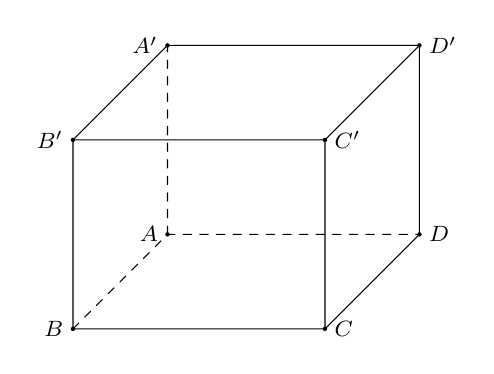
\begin{tikzpicture}[scale=0.8, font=\footnotesize, line join=round, line cap=round, >=stealth]
				\coordinate (A) at (0,0);
				\coordinate (B) at (-1.5,-1.5);
				\coordinate (C) at (2.5,-1.5);
				\coordinate (D) at (4,0);
				\coordinate (A') at (0,3);
				\coordinate (B') at (-1.5,1.5);
				\coordinate (C') at (2.5,1.5);
				\coordinate (D') at (4,3);
				\draw[dashed] (B)--(A)--(D) (A)--(A');
				\draw (A')--(B')--(C')--(D')--cycle;
				\draw (B')--(B)--(C)--(D)--(D') (C)--(C');
				\fill (A) circle (1pt) node[left] {$A$};
				\fill (B) circle (1pt) node[left] {$B$};
				\fill (C) circle (1pt) node[right] {$C$};
				\fill (D) circle (1pt) node[right] {$D$};
				\fill (A') circle (1pt) node[left] {$A'$};
				\fill (B') circle (1pt) node[left] {$B'$};
				\fill (C') circle (1pt) node[right] {$C'$};
				\fill (D') circle (1pt) node[right] {$D'$};
			\end{tikzpicture}
		\end{center}
		Diện tích toàn phần của hình hộp chữ nhật bằng tổng diện tích $6$ mặt của nó.\\
		Ta có công thức: $S_{\text{tp}} = 2(AB \cdot AD + AB \cdot AA' + AD \cdot AA')$.\\
		Thay các giá trị vào ta được
		\begin{eqnarray*}
			S_{\text{tp}}&= & 2(a \cdot 2a + a \cdot 2a + 2a \cdot 2a)\\
			&=& 2(2a^2 + 2a^2 + 4a^2)\\
			&= & 16a^2.
		\end{eqnarray*}
	}
\end{ex}

\begin{ex}%[2D1H1-2]%[TDMZZ19]%[Trần Văn Thiện, Nguyễn Sơn Thành]
	\immini{
		Cho đồ thị hàm số $y = f'(x)$ như hình vẽ bên dưới. Hỏi hàm số $f(x)$ nghịch biến trên khoảng nào dưới đây?
		\choice
		{$(5; 7)$}
		{$(-\infty; -5)$}
		{\True $(-5; 4)$}
		{$(-4; 5)$}
	}{
		\begin{tikzpicture}[
			>=stealth,
			line join=round,
			xscale=0.6, 
			every node/.style={font=\normalsize},
			declare function={
				f(\x)= (\x<0)*(-0.0008*(\x+5)*(\x)^2*(\x-4)*(\x-7))
				+(\x>=0)*(-0.0032*(\x+5)*(\x)^2*(\x-4)*(\x-7));
				xmin=-6.5;
				xmax=8.5;
				ymin=-2;
				ymax=3;
			}
			]
			\draw[-Stealth]
			(xmin,0)--(xmax,0) node[below] {$x$};
			\draw[-Stealth]
			(0,ymin)--(0,ymax) node[shift={(-6pt,-5pt)}] {$y$};
			\begin{scope}
				\clip (xmin,ymin) rectangle (xmax,ymax);
				\draw[
				smooth,
				samples=300,
				domain=xmin:xmax,
				postaction={
					decorate,
					decoration={
						markings,
						mark=at position 0.78 with {
							\node[sloped,above] {$f'(x)$};
						}
					}
				}
				]
				plot (\x,{f(\x)});
			\end{scope}
			\fill (-5,0) circle (1pt);
			\node[shift={(-135:10pt)}] at (-5,0) {$-5$};		
			\fill (0,0) circle (1pt);
			\node[shift={(135:10pt)}] at (0,0) {$O$};		
			\fill (4,0) circle (1pt);
			\node[shift={(135:10pt)}] at (4,0) {$4$};		
			\fill (7,0) circle (1pt);
			\node[shift={(-135:10pt)}] at (7,0) {$7$};		
		\end{tikzpicture}
	}
	\loigiai{
		Dựa vào đồ thị của hàm số $y = f'(x)$, ta thấy:\\
		$f'(x) \le 0 \Leftrightarrow \hoac{&-5 \le x \le 4\\&x \ge 7.}$\\ Dấu $=$ xảy ra tại các điểm $x=-5$, $x=0$, $x=4$, $x=7$.\\
		Do đó hàm số $y = f(x)$ nghịch biến trên các khoảng $(-5; 4)$ và $(7; +\infty)$.\\
		Đối chiếu với các đáp án, ta thấy khoảng $(-5; 4)$ thỏa mãn.
	}
\end{ex}

\begin{ex}%[2H5N1-1]%[TDMZZ19]%[Trần Văn Thiện, Nguyễn Sơn Thành]
	Trong không gian với hệ trục tọa độ $Oxyz$, cho mặt phẳng $(P) \colon 2x - y + 2z - 5 = 0$. Điểm nào dưới đây nằm trên $(P)$?
	\choice
	{\True $(1; -1; 1)$}
	{$(1; 1; 1)$}
	{$(0; 1; 2)$}
	{$(2; 1; -3)$}
	\loigiai{
		Thay tọa độ các điểm vào phương trình mặt phẳng $(P)$, ta có\\
		Với điểm $(1; -1; 1)$, ta có $2\cdot 1 - (-1) + 2\cdot 1 - 5 = 2 + 1 + 2 - 5 = 0$ (thỏa mãn).\\
		Vậy điểm $(1; -1; 1)$ nằm trên mặt phẳng $(P)$.
	}
\end{ex}

\begin{ex}%[2D1H2-1]%[TDMZZ19][Trần Văn Thiện, Nguyễn Sơn Thành]
	Hàm số $f(x) = x^4 + 4x - 1$ sẽ
	\choice
	{\True đạt cực tiểu tại $x = -1$}
	{đạt cực đại tại $x = -1$}
	{có giá trị cực tiểu bằng $-5$}
	{có giá trị cực đại bằng $-4$}
	\loigiai{
		Tập xác định $\mathscr{D} = \mathbb{R}$.\\
		Ta có $f'(x) = 4x^3 + 4$. Cho $f'(x) = 0 \Leftrightarrow 4x^3 + 4 = 0 \Leftrightarrow x = -1$.\\
		Bảng biến thiên
		\begin{center}
			
\begin{tikzpicture}
				\tkzTabInit[nocadre=true, lgt=1.2, espcl=3, deltacl=0.5]
				{$x$/0.7, $f'(x)$/0.7, $f(x)$/2}
				{$-\infty$, $-1$, $+\infty$}
				\tkzTabLine{, -, 0, +, }
				\tkzTabVar{+/$+\infty$, -/$-4$, +/$+\infty$}
			\end{tikzpicture}
		\end{center}
		Dựa vào bảng biến thiên, hàm số đạt cực tiểu tại $x = -1$ và giá trị cực tiểu là $y_{\text{CT}} = -4$.
	}
\end{ex}

\begin{ex}%[2D4H3-1]%[TDMZZ19]%[Trần Văn Thiện, Nguyễn Sơn Thành]
	Cho hình phẳng $(H)$ giới hạn bởi các đường $f(x)=\mathrm{e}^x+x$, $g(x)=\mathrm{e}+x$, trục tung $Oy$. Diện tích hình phẳng $(H)$ bằng
	\choice
	{$2$}
	{$\dfrac{1}{2}$}
	{\True $1$}
	{$\dfrac{\sqrt{3}}{2}$}
	\loigiai{
		Phương trình hoành độ giao điểm của hai đồ thị hàm số là
		\[\mathrm{e}^x+x=\mathrm{e}+x \Leftrightarrow \mathrm{e}^x=\mathrm{e} \Leftrightarrow x=1.\]
		Trục tung $Oy$ có phương trình là $x=0$.\\
		Diện tích hình phẳng $(H)$ là
		\[S=\displaystyle\int\limits_{0}^{1}\left|\mathrm{e}^x+x-(\mathrm{e}+x)\right|\mathrm{\,d}x=\displaystyle\int\limits_{0}^{1}\left|\mathrm{e}^x-\mathrm{e}\right|\mathrm{\,d}x.\]
		Vì với mọi $x \in [0;1]$ ta có $\mathrm{e}^x \le \mathrm{e}$ nên $\left|\mathrm{e}^x-\mathrm{e}\right| = \mathrm{e}-\mathrm{e}^x$.\\
		Do đó $S=\displaystyle\int\limits_{0}^{1}(\mathrm{e}-\mathrm{e}^x)\mathrm{\,d}x = (\mathrm{e}x-\mathrm{e}^x)\Big|_0^1 = (\mathrm{e}\cdot 1-\mathrm{e}^1)-(\mathrm{e}\cdot 0-\mathrm{e}^0) = 0-(-1) = 1$.
	}
\end{ex}

\begin{ex}%[2D4H2-1]%[TDMZZ19]%[Trần Văn Thiện, Nguyễn Sơn Thành]
	Cho biết $\displaystyle\int\limits_{0}^{\frac{\pi}{2}}\left[3f(x)-\sin x\right]\mathrm{\,d}x=4$. Giá trị của $\displaystyle\int\limits_{0}^{\frac{\pi}{2}}f(x)\mathrm{\,d}x$ bằng
	\choice
	{$1$}
	{$\dfrac{2}{3}$}
	{\True $\dfrac{5}{3}$}
	{$2\pi$}
	\loigiai{
		Ta có $\displaystyle\int\limits_{0}^{\frac{\pi}{2}}\left[3f(x)-\sin x\right]\mathrm{\,d}x=4 \Leftrightarrow 3\displaystyle\int\limits_{0}^{\frac{\pi}{2}}f(x)\mathrm{\,d}x - \displaystyle\int\limits_{0}^{\frac{\pi}{2}}\sin x\mathrm{\,d}x = 4$.\\
		Mà $\displaystyle\int\limits_{0}^{\frac{\pi}{2}}\sin x\mathrm{\,d}x = (-\cos x)\Big|_0^{\frac{\pi}{2}} = -\cos\dfrac{\pi}{2}-(-\cos 0) = 0-(-1) = 1$.\\
		Suy ra $3\displaystyle\int\limits_{0}^{\frac{\pi}{2}}f(x)\mathrm{\,d}x - 1 = 4 \Leftrightarrow 3\displaystyle\int\limits_{0}^{\frac{\pi}{2}}f(x)\mathrm{\,d}x = 5 \Leftrightarrow \displaystyle\int\limits_{0}^{\frac{\pi}{2}}f(x)\mathrm{\,d}x = \dfrac{5}{3}$.
	}
\end{ex}

\begin{ex}%[2H5H1-3]%[TDMZZ19]%[Trần Văn Thiện, Nguyễn Sơn Thành]
	Trong không gian $Oxyz$, cho ba điểm có tọa độ $A(2;0;-1)$, $B(1;2;2)$, $C(0;3;1)$. Mặt phẳng $(P)$ đi qua điểm $A$ và vuông góc với đường thẳng $BC$ có phương trình là
	\choice
	{$2x+y-2=0$}
	{\True $x-y+z-1=0$}
	{$x+z-1=0$}
	{$x-2y-2=0$}
	\loigiai{
		Ta có $\overrightarrow{BC}=(-1;1;-1)$.\\
		Mặt phẳng $(P)$ vuông góc với đường thẳng $BC$ nên nhận vectơ chỉ phương của đường thẳng $BC$ làm vectơ pháp tuyến.\\
		Suy ra $(P)$ có một vectơ pháp tuyến là $\overrightarrow{n}=(1;-1;1)$ (chọn vectơ cùng phương với $\overrightarrow{BC}$).\\
		Mặt phẳng $(P)$ đi qua điểm $A(2;0;-1)$ và có vectơ pháp tuyến $\overrightarrow{n}=(1;-1;1)$ có phương trình là
		\[1(x-2)-1(y-0)+1(z+1)=0 \Leftrightarrow x-y+z-1=0.\]
	}
\end{ex}

\begin{ex}%[2H2H1-3]%[TDMZZ19]%[Trần Văn Thiện, Nguyễn Sơn Thành]
	\immini{
		Cho hình lập phương $ABCD. A'B'C'D'$ có cạnh bằng $3$. Hãy tính $\left(\overrightarrow{AB}+\overrightarrow{CC'}\right)\cdot \overrightarrow{CD'}$.
		\choice
		{$3$}
		{$9$}
		{\True $0$}
		{$3\sqrt{3}$}
	}{
		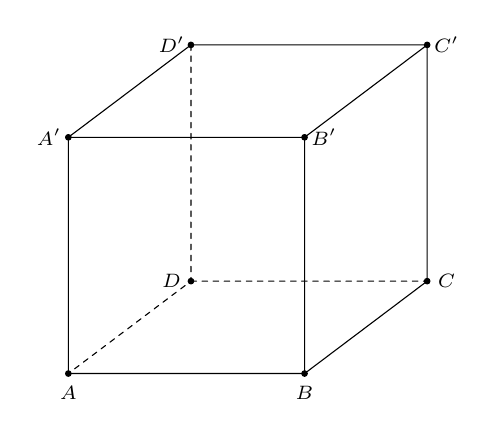
\begin{tikzpicture}[declare function={r=3;}, font=\footnotesize, line join=round, line cap=round, >=stealth]
			\path (0:0) coordinate (A)
			(0:r) coordinate (B)
			++(37:{0.65*r}) coordinate (C)
			++(180:r) coordinate (D)
			\foreach \x in {A,B,C,D}{(\x)++(90:r) coordinate (\x')};
			\draw[dash pattern=on 2pt off 2 pt] (D')--(D)--(A) (D)--(C);
			\draw (A)--(B)--(C) (A)--(A') (B)--(B') (C)--(C')(A')--(B')--(C')--(D')--cycle;
			\foreach \t/\g in {A/-90,B/-90,C/0,D/180,A'/180,B'/0,C'/0,D'/180}{
				\draw[fill=black] (\t) circle (1pt) node[shift={(\g:7pt)},font=\scriptsize]{$ \t $};
			}
		\end{tikzpicture}
	}
	\loigiai{
		Ta có $\overrightarrow{CC'} = \overrightarrow{BB'}$ (do $BCC'B'$ là hình chữ nhật).\\
		Suy ra $\overrightarrow{AB}+\overrightarrow{CC'} = \overrightarrow{AB}+\overrightarrow{BB'} = \overrightarrow{AB'}$.\\
		Lại có $\overrightarrow{CD'} = \overrightarrow{BA'}$ (do tứ giác $BCD'A'$ là hình bình hành nên $\overrightarrow{CD'}=\overrightarrow{BA'}$).\\
		Mặt khác, $ABB'A'$ là hình vuông nên hai đường chéo $AB'$ và $BA'$ vuông góc với nhau.\\
		Do đó $\overrightarrow{AB'} \cdot \overrightarrow{BA'} = 0$.\\
		Vậy $\left(\overrightarrow{AB}+\overrightarrow{CC'}\right)\cdot \overrightarrow{CD'} = \overrightarrow{AB'} \cdot \overrightarrow{BA'} = 0$.
	}
\end{ex}

\begin{ex}%[1D5H1-3]%[TDMZZ19]%[Trần Văn Thiện, Nguyễn Sơn Thành]
	Cho hai mẫu số liệu $M_1$, $M_2$ với bảng tần số ghép nhóm như sau:
	\begin{center}
		\textbf{Nhóm $\boldsymbol{M_1}$}
		\begin{tabular}{|c|c|c|c|c|c|c|}
			\hline
			Nhóm & $[8;10)$ & $[10;12)$ & $[12;14)$ & $[14;16)$ & $[16;18)$ & $[18;20)$ \\
			\hline
			Tần số & $6$ & $6$ & $4$ & $8$ & $6$ & $7$ \\
			\hline
		\end{tabular}
	\end{center}
	\begin{center}
		\textbf{Nhóm $\boldsymbol{M_2}$}
		\begin{tabular}{|c|c|c|c|c|c|c|}
			\hline
			Nhóm & $[8;10)$ & $[10;12)$ & $[12;14)$ & $[14;16)$ & $[16;18)$ & $[18;20)$ \\
			\hline
			Tần số & $6$ & $6$ & $8$ & $4$ & $6$ & $7$ \\
			\hline
		\end{tabular}
	\end{center}
	Hãy so sánh $\overline{x_1}$, $\overline{x_2}$ lần lượt là trung bình cộng của hai mẫu số liệu $M_1$, $M_2$?
	\choice
	{\True $\overline{x_1}>\overline{x_2}$}
	{$\overline{x_1}<\overline{x_2}$}
	{$\overline{x_1}=\overline{x_2}$}
	{$\overline{x_1}=3\overline{x_2}-4$}
	\loigiai{
		Giá trị đại diện của các nhóm $[8;10)$, $[10;12)$, $[12;14)$, $[14;16)$, $[16;18)$, $[18;20)$ lần lượt là $9$; $11$; $13$; $15$; $17$; $19$.\\
		Kích thước của mẫu số liệu $M_1$ là $n_1 = 6+6+4+8+6+7 = 37$.\\
		Kích thước của mẫu số liệu $M_2$ là $n_2 = 6+6+8+4+6+7 = 37$.\\
		Trung bình cộng của mẫu số liệu $M_1$ là
		\[\overline{x_1} = \dfrac{6\cdot 9 + 6\cdot 11 + 4\cdot 13 + 8\cdot 15 + 6\cdot 17 + 7\cdot 19}{37} = \dfrac{527}{37}.\]
		Trung bình cộng của mẫu số liệu $M_2$ là
		\[\overline{x_2} = \dfrac{6\cdot 9 + 6\cdot 11 + 8\cdot 13 + 4\cdot 15 + 6\cdot 17 + 7\cdot 19}{37} = \dfrac{519}{37}.\]
		Do $\dfrac{527}{37} > \dfrac{519}{37}$ nên $\overline{x_1} > \overline{x_2}$.
	}
\end{ex}
\cauds
\begin{ex}%[2D1V5-8]%[Dương Công Tạo]
	Quan sát sự phát triển của một quần thể vi khuẩn trong môi trường nuôi cấy hạn chế, cho ta kết quả:
	\begin{itemize}
		\item[ ]{\bf Giai đoạn 1} (từ $t=0$ đến $t=4$ giờ): Số lượng vi khuẩn tăng trưởng theo hàm mũ $N(t) = 60\mathrm{e}^{0{,}5t}$ (với $t$ tính bằng giờ, $N$ tính bằng nghìn cá thể).
		\item[ ]{\bf Giai đoạn 2} (sau $4$ giờ): Do nguồn dinh dưỡng cạn kiệt, tốc độ tăng trưởng giảm dần. Từ thời điểm này, số lượng vi khuẩn tuân theo hàm số $M(t) = A-B\mathrm{e}^{-0{,}4t}$.
	\end{itemize}
	Biết tốc độ tăng trưởng của quần thể vi khuẩn này là một hàm liên tục trên $t \in [0;+\infty)$.
	\choiceTF
	{Số lượng vi khuẩn ban đầu là $60$ con}
	{$B=75\mathrm{e}^2$}
	{\True $A=135\mathrm{e}^2$}
	{Sau khoảng thời gian rất lớn số lượng vi khuẩn đạt ổn định $999$ nghìn con (tính theo đơn vị nghìn và làm tròn kết quả đến hàng đơn vị)}
	\loigiai{
		Ta có
		\begin{itemize}
			\item Giai đoạn $1$, (từ $t=0$ đến $t=4$ giờ), ta có $N'(t) = 30\mathrm{e}^{0{,}5t}$.
			\item Giai đoạn $2$, (sau $4$ giờ), ta có $M'(t) = 0{,}4B\mathrm{e}^{-0{,}4t}$.
		\end{itemize}
		\begin{itemchoice}
			\itemch Số lượng vi khuẩn ban đầu là $N(0)=60\mathrm{e}^{0{,}5\cdot 0}=60$ (nghìn cá thể).
			\itemch Do tốc độ tăng trưởng của quần thể vi khuẩn này là một hàm liên tục trên $t \in [0;+\infty)$ nên nó liên tục tại $x=4\Leftrightarrow \lim\limits_{t\to4^-}N'(t)=\lim\limits_{t\to4^+}M'(t)\Leftrightarrow 30\mathrm{e}^{0{,}5\cdot4}=0{,}4B\mathrm{e}^{-0{,}4\cdot4}\Leftrightarrow B=75\mathrm{e}^{3{,}6}$.
			\itemch Do tốc độ tăng trưởng của quần thể vi khuẩn này là một hàm liên tục trên $t \in [0;+\infty)$ nên số lượng vi khuẩn $N(t)$ và $M(t)$ cũng liên tục trên $t \in [0;+\infty)$ nên nó liên tục tại $x=4$ \[\Leftrightarrow \lim\limits_{t\to4^-}N(t)=\lim\limits_{t\to4^+}M(t)\Leftrightarrow 60\mathrm{e}^{0{,}5\cdot4}=A-75\mathrm{e}^{3{,}6}\cdot\mathrm{e}^{-0{,}4\cdot4}\Leftrightarrow A=135\mathrm{e}^{2}.\]
			\itemch \lq\lq Sau khoảng thời gian rất lớn\rq\rq\, tương ứng với $t \to +\infty$.\\
			Số lượng vi khuẩn khi đó là \[\lim\limits_{t \to +\infty} M(t) = \lim\limits_{t \to +\infty}\left(A - B\mathrm{e}^{-0{,}4t}\right)= A = 135\mathrm{e}^2\approx 997{,}52\text{ (nghìn con)}.\]
		\end{itemchoice}
	}
\end{ex}

\begin{ex}%[2D6V2-2]%[TDMZZ19]%[Hà Văn Hảo]
	Ở một tỉnh có mở một cuộc trưng cầu dân ý, kết quả cho thấy có $45\%$ cử tri tham gia trả lời sẽ bầu cho ứng cử viên X. Sau cuộc bầu cử, tất cả cử tri từng tham gia cuộc trưng cầu dân ý đều phản hồi lại kết quả mình đã bầu chọn. Các phản hồi cho thấy trong số các cử tri từng trả lời sẽ bầu cho ứng cử viên X chỉ có $80\%$ đã thực sự bầu cho X, trong số các cử tri từng trả lời sẽ không bầu cho ứng cử viên X lại có $30\%$ đã bầu cho ứng cử viên X. Chọn ra một trong những người tham gia cuộc trưng cầu dân ý.
	\choiceTF
	{\True Xác suất chọn được cử tri đã trả lời sẽ bầu cho ứng cử viên X là $0{,}45$}
	{Xác suất chọn được cử tri thật sự không bầu cho ứng cử viên X là $0{,}625$}
	{\True Xác suất chọn được cử tri thật sự không bầu cho ứng cử viên X, nếu đã biết cử tri này trả lời sẽ bầu cho ứng cử viên X là $0{,}2$}
	{\True Xác suất để chọn được cử tri đã \lq\lq nói một đằng làm một nẻo\rq\rq \ là $0{,}255$}
	\loigiai{
		Gọi $A$ là biến cố \lq\lq Cử tri trả lời sẽ bầu cho ứng cử viên X\rq\rq.\\
		Khi đó $\overline{A}$ là biến cố \lq\lq Cử tri trả lời sẽ không bầu cho ứng cử viên X\rq\rq.\\
		Gọi $B$ là biến cố \lq\lq Cử tri thực sự bầu cho ứng cử viên X\rq\rq.\\
		Khi đó $\overline{B}$ là biến cố \lq\lq Cử tri thực sự không bầu cho ứng cử viên X\rq\rq.\\
		Theo giả thiết, ta có các xác suất sau
		\allowdisplaybreaks
		\begin{eqnarray*}
			&&\mathrm{P}(A) = 45\% = 0{,}45 \Rightarrow \mathrm{P}(\overline{A}) = 1 - 0{,}45 = 0{,}55. \\
			&&\mathrm{P}(B|A) = 80\% = 0{,}8 \Rightarrow \mathrm{P}(\overline{B}|A) = 1 - 0{,}8 = 0{,}2. \\
			&&\mathrm{P}(B|\overline{A}) = 30\% = 0{,}3 \Rightarrow \mathrm{P}(\overline{B}|\overline{A}) = 1 - 0{,}3 = 0{,}7.
		\end{eqnarray*}
		\begin{itemchoice}
			\itemch Xác suất chọn được cử tri đã trả lời sẽ bầu cho ứng cử viên X chính là $\mathrm{P}(A) = 0{,}45$.
			\itemch Xác suất cử tri thực sự bầu cho X theo công thức xác suất toàn phần là
			\allowdisplaybreaks
			\begin{eqnarray*}
				\mathrm{P}(B) &=& \mathrm{P}(A) \cdotp \mathrm{P}(B|A) + \mathrm{P}(\overline{A}) \cdotp \mathrm{P}(B|\overline{A}) \\
				&=& 0{,}45 \cdotp 0{,}8 + 0{,}55 \cdotp 0{,}3 \\
				&=& 0{,}36 + 0{,}165 = 0{,}525.
			\end{eqnarray*}
			Xác suất cử tri thực sự không bầu cho X là
			\[\mathrm{P}(\overline{B}) = 1 - \mathrm{P}(B) = 1 - 0{,}525 = 0{,}475. \]
			\itemch Đây là xác suất có điều kiện $\mathrm{P}(\overline{B}|A)$. Theo tính chất của xác suất có điều kiện
			\[ \mathrm{P}(\overline{B}|A) = 1 - \mathrm{P}(B|A) = 1 - 0{,}8 = 0{,}2. \]
			\itemch Cử tri \lq\lq nói một đằng làm một nẻo\rq\rq \ khi họ trả lời bầu nhưng thực sự không bầu, hoặc trả lời không bầu nhưng thực sự có bầu.\\
			Biến cố này là $C = (A \cap \overline{B}) \cup (\overline{A} \cap B)$.
			\allowdisplaybreaks
			\begin{eqnarray*}
				\mathrm{P}(C) &=& \mathrm{P}(A \cap \overline{B}) + \mathrm{P}(\overline{A} \cap B) \\
				&=& \mathrm{P}(A) \cdotp \mathrm{P}(\overline{B}|A) + \mathrm{P}(\overline{A}) \cdotp \mathrm{P}(B|\overline{A}) \\
				&=& 0{,}45 \cdotp 0{,}2 + 0{,}55 \cdotp 0{,}3 \\
				&=& 0{,}09 + 0{,}165 = 0{,}255.
			\end{eqnarray*}
		\end{itemchoice}
	}
\end{ex}

\begin{ex}%[2D4V3-4]%[TDMZZ19]%[Văn Minh Thoại]
	\immini[thm]{
		Trong không gian $Oxyz$ có đơn vị dài trên mỗi trục là mét, cho hình phẳng $(H)$ được gạch chéo và tô màu như hình vẽ và nằm trong mặt phẳng $(Oyz)$, $(H)$ được giới hạn bởi parabol $(P)$ và hai đoạn $CD$, $C'D'$. Một hình không gian $(K)$ có hai đáy dạng như $(H)$ và có chiều cao bằng $2$. Một bể nước có dạng $(K)$, nhưng mặt $ABCD$ kín và được đặt ở bên dưới và mặt $A'B'C'D'$ để hở. Ban đầu bể $(K)$ chưa chứa gì. Ta dùng một vòi nước có lưu lượng không đổi bằng $0{,}02$ m$^3$/phút chảy vào bể.
		
	}{
		\begin{tikzpicture}[
			line join=round,line cap=round,every node/.append style={font=\footnotesize},>=stealth,scale=1.4,declare function={f (\x)=25/9*(\x)^2-1/5; tysoK=0.4; docong=2pt;},xscale=1.5,yscale=1.5]
			\path
			(0,0) coordinate (O)
			(-2,-2) coordinate (Z)
			(0.6,{f (0.6)}) coordinate (C')
			(-0.6,{f (-0.6)}) coordinate (D')
			({3*sqrt (5)/25},0) coordinate (C)
			($(O)!-1!(C)$) coordinate (D)
			($(O)!0.75!(Z)$) coordinate (Ab)
			($(C)+(Ab)-(O)$) coordinate (B)
			($(D)+(Ab)-(O)$) coordinate (A)
			($(C')+(B)-(C)$) coordinate (B')
			($(D')+(A)-(D)$) coordinate (A')
			($(B)!tysoK!(C)$) coordinate (B1)
			($(B1)+(B')-(B)$) coordinate (B2)
			($(A)!tysoK!(D)$) coordinate (A1)
			($(A1)+(A')-(A)$) coordinate (A2);
			\fill[cyan!20]
			(D')--(C')--
			plot[samples=150,smooth,domain=0.6:{3*sqrt (5)/25}] (\x,{f (\x)})--
			(C)--(D)--
			plot[samples=150,smooth,domain={-3*sqrt (5)/25}:-0.6] (\x,{f (\x)})
			--cycle;
			\fill[blue!10] (D)--(C)--(B)--(A)--cycle;
			\fill[magenta!20,draw=black] (B').. controls ([xshift=docong]$(B')!0.35!(B)$) and ([xshift=docong]$(B')!0.65!(B)$).. (B)--(A)--(A).. controls ([xshift=-docong]$(A)!0.35!(A')$) and ([xshift=-docong]$(A)!0.65!(A')$).. (A')--cycle;
			
			\draw[->] (C)--(2,0) node[shift=(-110:0.2)] {$x$};
			\draw[->] (0,0.8)--(0,2) node[shift=(-150:0.2)] {$y$};
			\draw[->] (Ab)--(Z) node[shift=(-150:0.2)] {$z$};
			\draw plot[samples=150,smooth,domain=-0.8:-0.6] (\x,{f (\x)});
			\draw[dashed] plot[samples=150,smooth,domain=-0.6:{3*sqrt (5)/25}] (\x,{f (\x)});
			\draw plot[samples=150,smooth,domain={3*sqrt (5)/25}:0.8] (\x,{f (\x)});
			\draw
			(A')--(D')--(C')--(B')
			(B)--(A)
			(B)--(C)
			(B2)--(B1)
			(A')--(B')
			(A2)--(B2);
			\draw[dashed]
			(A)--(D)
			(B1)--(A1)--(A2)
			(C)--++(-1,0)
			(0,0.8)--++(0,-1.5)
			(O)--(Ab);
			\draw[<-] ($(A2)!0.3!(B2)+(0,-0.3)$)--++(-1,0.7) node[above] {$(K)$};
			\draw[<->] (0.85,0)--(0.85,{f (0.6)}) node[sloped,pos=0.5,below] {$0{,}8$};
			\draw[<->] ($(D')+(0,0.2)$)--($(C')+(0,0.2)$) node[sloped,pos=0.7,above] {$1{,}2$};
			\foreach \t/\g in {O/50,C/-30,D/160,B/0,A/180,C'/0,D'/180,B'/100,A'/180}{
				\draw[fill,ball color=red] (\t) circle (0.6pt)
				node[shift={(\g:3mm)}]{$\t$};
			}
			\node[below] at (Ab) {$2$};
			\node[shift=(-25:0.4)] at (0,-0.2) {$-0{,}2$};
			\node at ($(C)+(-0.1,0.6)$) {$(H)$};
			\node at ($(D')+(-0.4,0.6)$) {$(P)$};
		\end{tikzpicture}
	}
	\choiceTF
	{\True Phương trình parabol $(P)$ là $z=\dfrac{25}{9}y^2-0{,}2$}
	{\True Diện tích hình phẳng $(H)$ bằng $0{,}73$ m$^2$ \textit{(làm tròn đến hàng phần trăm)}}
	{\True Thời gian để nước chảy đầy bể $(K)$ là $72{,}8$ phút \textit{(thời gian được tính theo phút và làm tròn đến hàng phần mười)}}
	{\True Sau khi nước chảy được $60$ phút thì chiều cao của mực nước so với đáy $ABCD$ bằng $0{,}69$ m \textit{(làm tròn kết quả đến hàng phần trăm)}}
	\loigiai{
		\begin{center}
			\begin{tikzpicture}[
				line join=round,line cap=round,every node/.append style={font=\footnotesize},>=stealth,scale=1.4,declare function={f (\x)=25/9*(\x)^2-1/5;},xscale=1.5,yscale=1.5]
				\clip (-1,-0.5) rectangle (1.55,2);
				\path
				(0,0) coordinate (O)
				(-2,-2) coordinate (Z)
				(0.6,{f (0.6)}) coordinate (C')
				(-0.6,{f (-0.6)}) coordinate (D')
				({3*sqrt (5)/25},0) coordinate (C)
				($(O)!-1!(C)$) coordinate (D);
				\fill[cyan!20] (D')--(C')-- plot[samples=150,smooth,domain=0.6:{3*sqrt (5)/25}] (\x,{f (\x)})--(C)--(D)--plot[samples=150,smooth,domain={-3*sqrt (5)/25}:-0.6] (\x,{f (\x)})
				--cycle;
				\draw[->] (-1,0)--(1.5,0) node[shift=(-110:0.2)] {$y$};
				\draw[->] (0,-0.5)--(0,2) node[shift=(-150:0.2)] {$z$};
				\draw plot[samples=150,smooth,domain=-0.8:0.8] (\x,{f (\x)});
				\foreach \t/\g in {O/40,C/-30,D/150,C'/0,D'/180}{
					\draw[fill,ball color=red] (\t) circle (0.4pt) node[shift={(\g:9pt)},font=\scriptsize]{$\t$}; }
				\fill[ball color=red] (0,-0.2) circle (0.5pt) node[shift=(-20:0.5)]{$-0{,}2$};
				\fill[ball color=red] (0,0.8) circle (0.5pt) node[shift=(20:0.5)]{$0{,}8$};
			\end{tikzpicture}
		\end{center}
		\begin{itemchoice}
			\itemch Dựa vào hệ trục tọa độ $Oyz$, parabol $(P)$ có đỉnh nằm trên trục $Oz$ tại $I(0;-0{,}2)$ nên có phương trình dạng $z=ay^2-0{,}2$. \\
			Mặt khác, đoạn $C'D'=1{,}2$ và nằm ở độ cao $z=0{,}8$ nên điểm $C'(0{,}6; 0{,}8)$. \\
			Parabol đi qua $C'(0{,}6; 0{,}8)$ nên ta có
			\[0{,}8 = a(0{,}6)^2 - 0{,}2 \Leftrightarrow 1 = 0{,}36a \Leftrightarrow a = \dfrac{100}{36} = \dfrac{25}{9}.\]
			Vậy phương trình parabol $(P)$ là $z=\dfrac{25}{9}y^2-0{,}2$.
			\itemch Hình phẳng $(H)$ được giới hạn bởi đường thẳng $C'D'$ ($z=0{,}8$), đường thẳng $CD$ ($z=0$) và hai nhánh của parabol $(P)$. \\
			Từ phương trình $(P)\colon z=\dfrac{25}{9}y^2-0{,}2\Rightarrow y^2=\dfrac{9}{25}(z+0{,}2)\Rightarrow y=\pm\dfrac{3}{5}\sqrt{z+0{,}2}$. \\
			Do tính đối xứng qua trục $Oz$, diện tích hình phẳng $(H)$ được tính bằng tích phân theo biến $z$, khi đó
			\allowdisplaybreaks
			\begin{align*}
				S_{(H)} &= \displaystyle\int\limits_{0}^{0{,}8} 2|y| \mathrm{\,d}z = 2 \displaystyle\int\limits_{0}^{0{,}8} \dfrac{3}{5}\sqrt{z+0{,}2} \mathrm{\,d}z \\
				&= \dfrac{6}{5} \left.\left[ \dfrac{2}{3} (z+0{,}2)^{\tfrac{3}{2}} \right]\right|_0^{0{,}8}\\
				& = \dfrac{4}{5} \left( 1^{\tfrac{3}{2}} - 0{,}2^{\tfrac{3}{2}} \right) \\
				&= 0{,}8 \left( 1 - 0{,}2\sqrt{0{,}2} \right) \approx 0{,}73\mathrm{\,m}^2.
			\end{align*}
			\itemch Thể tích bể nước $(K)$ (dạng hình trụ đứng có đáy là hình phẳng $(H)$ và chiều cao $h=2$) là
			\[V = S_{(H)} \cdot h \approx 0{,}728448 \cdot 2 \approx 1{,}4569 \mathrm{\,m}^3.\]
			Thời gian để nước chảy đầy bể với lưu lượng $0{,}02$ m$^3$/phút là
			\[t = \dfrac{V}{0{,}02} \approx \dfrac{1{,}4569}{0{,}02} \approx 72{,}8\;\text{phút}.\]
			\itemch Sau khi nước chảy được $60$ phút, thể tích nước trong bể là
			\[V_{60} = 60 \cdot 0{,}02 = 1{,}2 \mathrm{\,m}^3.\]
			Bể đặt phần $ABCD$ ở dưới đáy (tương ứng $z=0$). Gọi $h_0$ là chiều cao mực nước so với đáy $ABCD$ ($0<h_0<0{,}8$). \\
			Thể tích nước lúc này tương ứng với hình lăng trụ có đáy là hình phẳng giới hạn từ $z=0$ đến $z=h_0$, khi đó
			\allowdisplaybreaks
			\begin{eqnarray*}
				&&V_{60} = \left( \displaystyle\int\limits_{0}^{h_0} 2 \cdot \dfrac{3}{5}\sqrt{z+0{,}2} \mathrm{\,d}z \right) \cdot 2 = 1{,}2\\
				&\Leftrightarrow&\displaystyle\int\limits_{0}^{h_0} \dfrac{6}{5}\sqrt{z+0{,}2} \mathrm{\,d}z = 0{,}6 \\
				&\Leftrightarrow & \dfrac{4}{5} \left( (h_0+0{,}2)^{\tfrac{3}{2}} - 0{,}2^{\tfrac{3}{2}} \right) = 0{,}6 \\
				&\Leftrightarrow & (h_0+0{,}2)^{\tfrac{3}{2}} - 0{,}2\sqrt{0{,}2} = 0{,}6 \cdot \dfrac{5}{4} \\
				&\Leftrightarrow & (h_0+0{,}2)^{\tfrac{3}{2}} = 0{,}75 + 0{,}2\sqrt{0{,}2}\\
				&\Leftrightarrow & h_0+0{,}2 = \left( 0{,}75 + 0{,}2\sqrt{0{,}2} \right)^{\tfrac{2}{3}}\\
				&\Rightarrow & h_0 \approx 0{,}69 \mathrm{\,m}.
			\end{eqnarray*}
			Vậy chiều cao mực nước là $0{,}69$ m.
		\end{itemchoice}
	}
\end{ex}

\begin{ex}%[2H5V3-2]%[TDMZZ19]%[Vũ Hồng Toàn]
	Trong không gian $Oxyz$, cho hai mặt cầu có phương trình lần lượt là $(S_1)\colon (x-2)^2 + y^2 + (z-3)^2 = 9$ và $(S_2)\colon (x+2)^2 + (y-2)^2 + (z+1)^2 = 25$.
	\choiceTF
	{\True Tâm của mặt cầu $(S_1)$ là $I_1(2;0;3)$, của mặt cầu $(S_2)$ là $I_2(-2;2;-1)$}
	{\True Thể tích của $(S_2)$ lớn hơn của $(S_1)$ một lượng bằng $411$ (làm tròn kết quả đến hàng đơn vị)}
	{Khoảng cách ngắn nhất giữa hai điểm nằm trên $(S_1)$ và $(S_2)$ là $2$}
	{\True Khoảng cách lớn nhất giữa hai điểm nằm trên $(S_1)$ và $(S_2)$ là $14$}
	\loigiai{
		\begin{itemchoice}
			\itemch Ta có
			\begin{itemize}
				\item Mặt cầu $\left(S_1\right)$ có tâm $I_1\left(2;0;3\right)$ và bán kính $R_1 = 3$.
				\item Mặt cầu $\left(S_2\right)$ có tâm $I_2\left(-2;2;-1\right)$ và bán kính $R_2 = 5$.
			\end{itemize}
			\itemch Thể tích của hai mặt cầu lần lượt là
			\begin{itemize}
				\item $V_1 = \dfrac{4}{3}\pi R_1^3 = \dfrac{4}{3}\pi \cdot 3^3 = 36\pi$.
				\item $V_2 = \dfrac{4}{3}\pi R_2^3 = \dfrac{4}{3}\pi \cdot 5^3 = \dfrac{500}{3}\pi$.
			\end{itemize}
			Hiệu thể tích của hai mặt cầu là:
			$V_2 - V_1 = \dfrac{500}{3}\pi - 36\pi \approx 410{,}5 \approx 411$.
			\itemch Khoảng cách giữa hai tâm $I_1$ và $I_2$ là
			$I_1I_2 = \sqrt{(-2-2)^2 + (2-0)^2 + (-1-3)^2} = 6$.\\
			Vì $|R_1 - R_2| = 2 < I_1I_2 = 6 < R_1 + R_2 = 8$, suy ra hai mặt cầu $\left(S_1\right)$ và $\left(S_2\right)$ cắt nhau.\\
			Do hai mặt cầu cắt nhau nên khoảng cách ngắn nhất giữa hai điểm nằm trên $\left(S_1\right)$ và $\left(S_2\right)$ bằng $0$.
			\itemch Khoảng cách lớn nhất giữa hai điểm nằm trên $(S_1)$ và $(S_2)$ là
			\[d_{\max} = I_1I_2 + R_1 + R_2 = 6 + 3 + 5 = 14.\]
		\end{itemchoice}
	}
\end{ex}
\caukq
\begin{ex}%[1H8V5-4]%[TDMZZ19]%[Lê Hồ Quang Minh]
	Cho khối chóp cụt đều $ABC. A'B'C'$ có độ dài các cạnh $AB = 4$, $A'B' = 8$, chiều cao bằng $6$. Hãy tính khoảng cách giữa hai đường thẳng $AB$ và $CC'$ \textit{(làm tròn kết quả đến hàng phần mười)}.
	\par
	\shortans[0]{3,2}
	\loigiai{
		Gọi $O$ và $O'$ lần lượt là tâm của hai đáy $ABC$ và $A'B'C'$.\\
		Từ giả thiết suy ra $OO'=6$.\\
		Gọi $S$ là giao điểm của các cạnh bên hình chóp cụt đều.\\
		Khi đó ta được $S. ABC$ và $S. A'B'C'$ là hình chóp tam giác đều.\\
		Vì $AB = \dfrac{1}{2}A'B'$ nên $A$, $B$, $C$ lần lượt là trung điểm của $SA'$, $SB'$, $SC'$.\\
		Do đó $O$ cũng là trung điểm của $SO'$.\\
		Suy ra $SO' = 12$.\\
		\textbf{Cách 1: Dành cho lớp 11}
		\immini{Ta có $\mathrm{d}(AB;CC') = \mathrm{d}(AB;SC)$.\\
			Trong hình chóp đều $S. ABC$ ta dựng hình thoi $ABCD$.\\
			Khi đó $\heva{&AB \parallel CD\\& CD \subset (SCD)} \Rightarrow AB \parallel (SCD)$.\\
			Suy ra $$\mathrm{d}(AB;SC)= \mathrm{d}(AB;(SCD))=\mathrm{d}(B;(SCD)) = \dfrac{3}{2}\cdot \mathrm{d}(O;(SCD)) = \dfrac{3}{2}OH.$$
			Xét tam giác $SOC$ vuông tại $O$ có $\heva{&SO = OO'=6\\&OC = \dfrac{2}{3}\cdot \dfrac{4\sqrt{3}}{2}=\dfrac{4\sqrt{3}}{3}.}$
			\[OH=\dfrac{SO \cdot OC}{\sqrt{SO^2 + OC^2}} = \dfrac{6 \cdot \dfrac{4\sqrt{3}}{3}}{\sqrt{6^2 + \dfrac{16}{3}}} =\dfrac{12\sqrt{31}}{31}.\]
			Vậy $\mathrm{d}(AB;CC') = \dfrac{18\sqrt{31}}{31} \approx 3{,}2$.
		}{\begin{tikzpicture}[scale=0.6, font=\footnotesize,line join=round, line cap=round, >=stealth]
				\path 
				(0,0) coordinate (A)
				++(-60:2) coordinate (C)
				(5,0) coordinate (B)
				($(B)!1/2!(C)$) coordinate (M)
				($(A)!2/3!(M)$) coordinate (O)
				($(O)+(0,6)$) coordinate (S)
				($(C)+(A)-(B)$) coordinate (D)
				($(S)!0.6!(C)$) coordinate (H)
				;
				\foreach \i in{B,C}{\draw (S)--(\i);};
				\draw (B)--(C)--(D)--(S);
				\draw[dashed] (A)--(S)--(O) (B)--(A)--(C)--(O)--(H) (A)--(D)--(B);
				\pic[draw,angle eccentricity=1.8,angle radius=2mm]{right angle=S--O--A} pic[draw,angle eccentricity=1.8,angle radius=2mm]{right angle=O--H--C};
				\foreach \i/\g in {S/90,A/150,C/-90,B/0,O/-90,D/180,H/180}
				\fill[black] (\i) circle(1pt)+(\g:4mm)node[scale=1]{$\i$};
		\end{tikzpicture}}
		\noindent\textbf{Cách 2: Dành cho lớp 12, sử dụng hệ trục tọa độ $Oxyz$}
		\immini{
			Chọn hệ trục tọa độ $Mxyz$ như hình vẽ.\\
			Ta có $A'\left(0;4\sqrt{3};0\right)$, $B'\left(4;0;0\right)$, $C'(-4;0;0)$, $S\left(0;\dfrac{4\sqrt{3}}{3};12\right)$.\\
			Từ đó suy ra $A\left(0;\dfrac{8\sqrt{3}}{3};6\right)$, $B\left(2;\dfrac{2\sqrt{3}}{3};6\right)$ và $C\left(-2;\dfrac{2\sqrt{3}}{3};6\right)$.
		}{
			\begin{tikzpicture}[scale=0.8, font=\footnotesize,line join=round, line cap=round, >=stealth]
				\path 
				(0,0) coordinate (A')
				++(-60:2) coordinate (B')
				(6,0) coordinate (C')
				($(B')!1/2!(C')$) coordinate (M)
				($(A')!2/3!(M)$) coordinate (O')
				($(O')+(0,6)$) coordinate (S)
				($(A')!1/2!(S)$) coordinate (A)
				($(B')!1/2!(S)$) coordinate (B)
				($(C')!1/2!(S)$) coordinate (C)
				(intersection of S--M and B--C) coordinate (I)
				(intersection of A--I and S--O') coordinate (O)
				($(M)!1.3!(A')$) coordinate (y)
				($(M)!1.3!(B')$) coordinate (x)
				($(M)+(0,7)$) coordinate (z)
				;
				\foreach \i in{A',B',C'}{\draw (S)--(\i);};
				\draw (A')--(B')--(C') (A)--(B)--(C);
				\draw[->] (A')--(y);
				\draw[->] (B')--(x);
				\draw[->] (M)--(z);
				\draw[dashed] (M)--(A')--(C') (S)--(O') (C)--(A)--(I);
				\pic[draw,angle eccentricity=1.8,angle radius=2mm]{right angle=A'--M--B'};
				\foreach \i/\g in {A'/-130,B'/-90,C'/0,S/90,M/-90,O'/-90,A/180,B/180,C/0,O/-160}
				\fill[black] (\i) circle(1pt)+(\g:4mm)node[scale=1]{$\i$};
				\foreach \i/\g in {x/90,y/90,z/90}
				\fill[black] (\i) circle(0.1pt)+(\g:4mm)node[scale=1]{$\i$};
		\end{tikzpicture}}
		\noindent Ta có $\heva{&\overrightarrow{AB}=\left(2;-2\sqrt{3};0\right)\\ &\overrightarrow{CC'} = \left(-2;-\dfrac{2\sqrt{3}}{3};-6\right)\\&\overrightarrow{AC}=\left(-2;-2\sqrt{3};0\right)}$ $\Rightarrow \heva{&\left[\overrightarrow{AB};\overrightarrow{CC'}\right] = \left(12\sqrt{3};12;-\dfrac{16\sqrt{3}}{3}\right)\\&\left[\overrightarrow{AB};\overrightarrow{CC'}\right]\cdot \overrightarrow{AC} = -48\sqrt{3}.}$\\
		Vậy $\mathrm{d}\left(AB;CC'\right) = \dfrac{\left|\left[\overrightarrow{AB};\overrightarrow{CC'}\right]\cdot \overrightarrow{AC}\right|}{\left|\left[\overrightarrow{AB};\overrightarrow{CC'}\right]\right|} = \dfrac{48\sqrt{3}}{\sqrt{432+144+\dfrac{256}{3}}} = \dfrac{18\sqrt{31}}{31} \approx 3{,}2$.
	}
\end{ex}

\begin{ex}%[2H2V2-6]%[Đề KSCL Ninh Bình 2025-2026]%[12]
	\immini{
		Cho tứ diện $ABCD$ đã biết độ dài $5$ cạnh cho như hình vẽ và một cạnh bằng $a$. Gieo ngẫu nhiên một con xúc xắc cân đối đồng chất hai lần liên tiếp, được tổng số chấm hai lần ta gán cho $a$. Hãy tính xác suất để thu được một hình tứ diện $ABCD$ hợp lí (\textit{không làm tròn ở các phép tính trung gian và làm tròn kết quả cuối cùng đến hàng phần trăm})?
	}{
		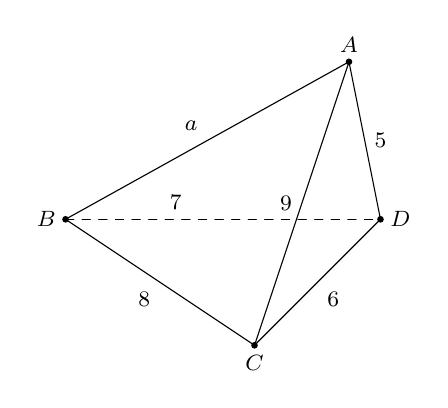
\begin{tikzpicture}[scale=0.8, font=\footnotesize, line join=round, line cap=round, >=stealth]
			\coordinate (B) at (0,0);
			\coordinate (D) at (5,0);
			\coordinate (C) at (3,-2);
			\coordinate (A) at (4.5,2.5);
			
			\draw (A) -- (B) node[midway, above left] {$a$};
			\draw (A) -- (C) node[midway, left] {$9$};
			\draw (A) -- (D) node[midway, right] {$5$};
			\draw (B) -- (C) node[midway, below left] {$8$};
			\draw (C) -- (D) node[midway, below right] {$6$};
			\draw[dashed] (B) -- (D) node[midway, above, pos=0.35] {$7$};
			
			\fill (A) circle (1.5pt) node[above] {$A$};
			\fill (B) circle (1.5pt) node[left] {$B$};
			\fill (C) circle (1.5pt) node[below] {$C$};
			\fill (D) circle (1.5pt) node[right] {$D$};
		\end{tikzpicture}
	}
	\par
	\shortans[0]{0,89}
	\loigiai{
		Ta gắn hệ trục tọa độ $Oxyz$ sao cho gốc tọa độ $O \equiv C(0;0;0)$.\\
		Vì $CD = 6$ nên ta có thể chọn $D(0;0;6)$ nằm trên tia $Oz$.\\
		Gọi tọa độ điểm $A$ là $A(x_A; y_A; z_A)$. Theo giả thiết ta có:
		\[\heva{& AC^2 = 9^2 \\ & AD^2 = 5^2} \Leftrightarrow \heva{& x_A^2 + y_A^2 + z_A^2 = 81 \\ & x_A^2 + y_A^2 + (z_A - 6)^2 = 25.}\]
		Trừ vế theo vế hai phương trình, ta được:
		\[z_A^2 - (z_A - 6)^2 = 56 \Leftrightarrow 12z_A - 36 = 56 \Leftrightarrow z_A = \dfrac{23}{3}.\]
		Suy ra $x_A^2 + y_A^2 = 81 - \left(\dfrac{23}{3}\right)^2 = \dfrac{200}{9}$.\\
		Do đó, điểm $A$ nằm trên đường tròn $(C_1)$ có tâm trên trục $Oz$, bán kính $R_A = \dfrac{10\sqrt{2}}{3}$ và thuộc mặt phẳng $z = \dfrac{23}{3}$.
		
		Tương tự, gọi tọa độ điểm $B$ là $B(x_B; y_B; z_B)$. Ta có:
		\[\heva{& BC^2 = 8^2 \\ & BD^2 = 7^2} \Leftrightarrow \heva{& x_B^2 + y_B^2 + z_B^2 = 64 \\ & x_B^2 + y_B^2 + (z_B - 6)^2 = 49.}\]
		Trừ vế theo vế hai phương trình, ta được:
		\[z_B^2 - (z_B - 6)^2 = 15 \Leftrightarrow 12z_B - 36 = 15 \Leftrightarrow z_B = \dfrac{17}{4}.\]
		Suy ra $x_B^2 + y_B^2 = 64 - \left(\dfrac{17}{4}\right)^2 = \dfrac{735}{16}$.\\
		Do đó, điểm $B$ nằm trên đường tròn $(C_2)$ có tâm trên trục $Oz$, bán kính $R_B = \dfrac{7\sqrt{15}}{4}$ và thuộc mặt phẳng $z = \dfrac{17}{4}$.
		
		Bình phương khoảng cách $AB$ được tính bởi:
		$AB^2 = (x_A - x_B)^2 + (y_A - y_B)^2 + (z_A - z_B)^2$.\\
		Ta có $(z_A - z_B)^2 = \left(\dfrac{23}{3} - \dfrac{17}{4}\right)^2 = \left(\dfrac{41}{12}\right)^2 = \dfrac{1681}{144}$.\\
		Gọi $A', B'$ lần lượt là hình chiếu vuông góc của $A, B$ xuống mặt phẳng $(Oxy)$. Khi đó $A', B'$ nằm trên hai đường tròn đồng tâm $O$, bán kính lần lượt là $R_A$ và $R_B$. Khoảng cách $(x_A - x_B)^2 + (y_A - y_B)^2$ chính là $A'B'^2$.\\
		Theo bất đẳng thức tam giác, ta luôn có $(R_A - R_B)^2 \le A'B'^2 \le (R_A + R_B)^2$.\\
		Để $A, B, C, D$ tạo thành một tứ diện hợp lí thì $4$ điểm này không đồng phẳng. Điều này tương đương với $A, B$ và trục $Oz$ (chứa $C, D$) không đồng phẳng. Khi đó $O, A', B'$ không thẳng hàng nên dấu bằng trong bất đẳng thức trên không xảy ra.
		\[\Rightarrow (R_A - R_B)^2 < A'B'^2 < (R_A + R_B)^2.\]
		Thay số vào, ta tính được khoảng chặn của $AB^2$:
		\allowdisplaybreaks
		\begin{align*}
			&AB^2 > \dfrac{1681}{144} + \left(\dfrac{10\sqrt{2}}{3} - \dfrac{7\sqrt{15}}{4}\right)^2 = \dfrac{11496 - 1680\sqrt{30}}{144} \approx 15{,}93 \Rightarrow AB > 3{,}99.\\
			&AB^2 < \dfrac{1681}{144} + \left(\dfrac{10\sqrt{2}}{3} + \dfrac{7\sqrt{15}}{4}\right)^2 = \dfrac{11496 + 1680\sqrt{30}}{144} \approx 143{,}73 \Rightarrow AB < 11{,}99.
		\end{align*}
		Vì $a = AB$ nên ta phải có $3{,}99 < a < 11{,}99$.\\
		Gieo ngẫu nhiên $2$ con xúc xắc, tổng số chấm $a \in \mathbb{N}$ và $2 \le a \le 12$. Kết hợp điều kiện trên, các giá trị hợp lệ là $a \in \{4; 5; 6; 7; 8; 9; 10; 11\}$.\\
		Các trường hợp $a$ không thỏa mãn là $a \in \{2; 3; 12\}$.
		\begin{itemize}
			\item $a = 2$: có $1$ kết quả là $(1; 1)$.
			\item $a = 3$: có $2$ kết quả là $(1; 2), (2; 1)$.
			\item $a = 12$: có $1$ kết quả là $(6; 6)$.
		\end{itemize}
		Tổng số kết quả không thỏa mãn là $1 + 2 + 1 = 4$.\\
		Không gian mẫu khi gieo $2$ con xúc xắc là $n(\Omega) = 6^2 = 36$.\\
		Số kết quả thuận lợi để được hình tứ diện hợp lí là $n(X) = 36 - 4 = 32$.\\
		Xác suất cần tìm là $P = \dfrac{32}{36} = \dfrac{8}{9} \approx 0{,}89$.
	}
\end{ex}

\begin{ex}%[2D1V3-6]%[TDMZZ19-19-TLN]
	Một doanh nghiệp $X$ chuyên kinh doanh xe gắn máy các loại. Hiện tại doanh nghiệp đang tập trung chiến lược vào kinh doanh loại xe $Y$ với chi phí mua vào một chiếc là $18$ triệu đồng và bán ra với giá $25$ triệu đồng. Với giá bán này thì số lượng xe mà khách hàng sẽ mua trong một năm là $200$ chiếc. Nhằm mục tiêu đẩy mạnh lượng tiêu thụ dòng xe đang ăn khách này, doanh nghiệp dự định giảm giá bán và theo đánh giá cho thấy nếu giảm $0{,}5$ triệu đồng mỗi chiếc xe thì số lượng xe bán ra trong một năm sẽ tăng thêm $20$ chiếc. Hãy xác định theo đơn vị triệu đồng, lợi nhuận lớn nhất mà doanh nghiệp này thu được.
	\par
	\shortans[0]{1440}
	\loigiai{
		Gọi $x$ là số lần giảm giá $0{,}5$ triệu đồng ($x \ge 0$).
		\begin{itemize}
			\item Giá bán mới là $25 - 0{,}5x$ (triệu đồng).
			\item Số lượng xe bán ra là $200 + 20x$ (chiếc).
			\item Lợi nhuận trên mỗi chiếc xe là $(25 - 0{,}5x) - 18 = 7 - 0{,}5x$ (triệu đồng).
		\end{itemize}
		Lợi nhuận thu được trong một năm là $f(x) = (7 - 0{,}5x)(200 + 20x)$, hay $f(x) = -10x^2 + 40x + 1\,400$.\\
		Ta có $f'(x)=-20x+40$, $f'(x)=0\Leftrightarrow x=2$.\\
		Bảng biến thiên
		\begin{center}
			
\begin{tikzpicture}
				\tkzTabInit[nocadre=false,lgt=1.2,espcl=2,deltacl=0.6]
				{$x$ /0.7, $f'(x)$/0.7,$f(x)$ /2}
				{$0$, $2$, $+\infty$}
				\tkzTabLine{,+,0,-,}
				\tkzTabVar {-/,+/$f(2)$,-/}
			\end{tikzpicture}
		\end{center}
		Suy ra, giá trị lớn nhất của lợi nhuận là $f(2) = -10\cdot 2^2 + 40\cdot 2 + 1\,400 = 1\,440$ (triệu đồng).
		\textit{Kiểm tra lại:}
		Giá bán mới: $25 - 0{,}5(2) = 24$ triệu đồng.
		Số lượng xe: $200 + 20(2) = 240$ chiếc.
		Lợi nhuận mỗi chiếc: $24 - 18 = 6$ triệu đồng.
		Tổng lợi nhuận: $240 \cdot 6 = 1\,440$ triệu đồng.
	}
\end{ex}

\begin{ex}%[2D6H2-2]%[TDMZZ19]%[Nguyễn Đức Tuấn Anh]
	Một thanh niên tên Hải đẹp trai, con nhà giàu cũng đến tuổi $3\text{x}$ mà vẫn ham chơi chưa lập gia đình. Một hôm, bố mẹ của Hải sắp xếp cho cậu gặp $12$ người con gái để gặp xem mặt đặt vấn đề lập gia đình. Bố mẹ Hải có chuẩn bị $12$ bí quyết tỏ tình thành công, mỗi bí quyết thành công với đúng một cô gái. Biết rằng, trong $12$ cô gái thì có $5$ cô chắc chắn đồng ý khi Hải tỏ tình. Nhưng Hải ham chơi và chỉ muốn gặp đúng một người cho xong việc rồi đi chơi. Chính vì vậy, Hải chọn ngẫu nhiên $7$ bí quyết mà bố mẹ đưa cho để đi xem mặt. Hải chọn ngẫu nhiên một trong $12$ cô gái để tỏ tình (bằng cách dùng $7$ bí quyết mang theo). Hãy tính xác suất để Hải tỏ tình thành công (\textit{làm tròn kết quả đến hàng phần trăm}).
	\par
	\shortans[0]{0,76}
	\loigiai{
		Gọi $A_1$ là biến cố \lq\lq Hải chọn trúng cô gái nằm trong số $5$ cô chắc chắn đồng ý\rq\rq.\\
		Gọi $A_2$ là biến cố \lq\lq Hải chọn trúng cô gái nằm trong số $7$ cô còn lại\rq\rq.\\
		Khi đó $A_1, A_2$ là một hệ biến cố đầy đủ và ta có $\mathrm{P}(A_1) = \dfrac{5}{12}$; $\mathrm{P}(A_2) = \dfrac{7}{12}$.\\
		Gọi $B$ là biến cố \lq\lq Hải tỏ tình thành công\rq\rq.
		\begin{itemize}
			\item Nếu Hải chọn trúng cô gái nằm trong nhóm $5$ cô chắc chắn đồng ý thì xác suất thành công là $1$. Suy ra $\mathrm{P}(B \mid A_1) = 1$.
			\item Nếu Hải chọn trúng cô gái nằm trong $7$ cô còn lại, để tỏ tình thành công thì trong $7$ bí quyết Hải mang theo phải chứa đúng bí quyết dành riêng cho cô gái đó. 
			Xác suất để xảy ra điều này là 
			\[\mathrm{P}(B \mid A_2) = \dfrac{\mathrm{C}_1^1 \cdot \mathrm{C}_{11}^6}{\mathrm{C}_{12}^7} = \dfrac{7}{12}.\]
		\end{itemize}
		Áp dụng công thức xác suất toàn phần, xác suất để Hải tỏ tình thành công là
		\allowdisplaybreaks
		\begin{align*}
			\mathrm{P}(B) &= \mathrm{P}(A_1) \cdot \mathrm{P}(B \mid A_1) + \mathrm{P}(A_2) \cdot \mathrm{P}(B \mid A_2) \\
			&= \dfrac{5}{12} \cdot 1 + \dfrac{7}{12} \cdot \dfrac{7}{12} = \dfrac{109}{144} \approx 0{,}76.
		\end{align*}
	}
\end{ex}

\begin{ex}%[2D4C3-4]%[TDMZZ19]%[Trương Tường]
	\immini[thm]{Cho một mặt bàn hình lục giác đều có cạnh bằng $126$\,cm. Để tạo thành một mặt bàn đẹp người ta vát ở $6$ góc bởi những phần parabol bằng nhau sao cho đỉnh của parabol cách tâm của mặt bàn $115$\,cm và parabol tiếp xúc với hai cạnh của hình lục giác đều ở mỗi góc bàn. Hãy tính diện tích mặt bàn sau khi đã vát theo đơn vị mét vuông (làm tròn kết quả đến hàng phần trăm)?}{
	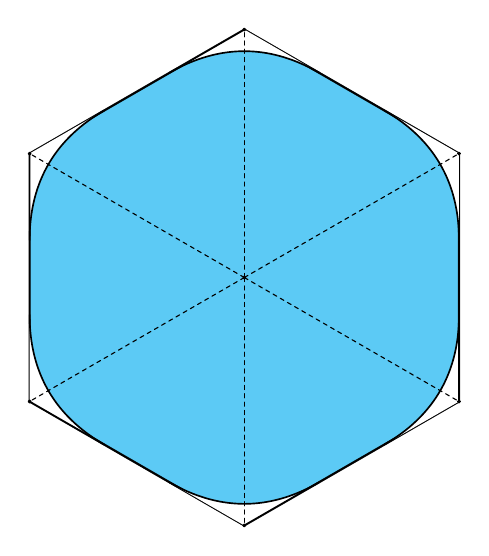
\begin{tikzpicture}[scale=0.025, >=stealth, line join=round, line cap=round, font=\footnotesize]
		\tikzset{declare function={a=126;f(\x)=115-(\x)^2/132;x0=22*sqrt(3);}}
		\path (0,0) coordinate (I)
		\foreach \x/\y in {0/A, 1/B, 2/C, 3/D, 4/E, 5/F}{
			(I)++({30+\x*60}:a) coordinate (\y)
		}
		;
		\draw [thick, fill=cyan!80, opacity=.8] (A)--(B)--(C)--(D)--(E)--(F)--cycle;
		\foreach \g in {0,60,...,300}{
			\begin{scope}[rotate=\g]
				\draw [semithick] (0,0)+(30:a)--+(90:a);
				\fill [smooth, samples=100, semithick, white] plot [domain={-22*sqrt(3)}:{22*sqrt(3)}] (\x, {f(\x)})--(0,a)--cycle;
				\draw [smooth, samples=100, semithick] plot [domain={-22*sqrt(3)}:{22*sqrt(3)}] (\x, {f(\x)});
			\end{scope}
		}
		\foreach \x in {A,B,C,D,E,F}{
			\draw [dash pattern=on 1.5pt off 1.5pt] (I)--(\x);
		}
		;
		\foreach \x in {A,B,C,D,E,F,I}{
			\draw [fill=black] (\x) circle (20pt);
		}
	\end{tikzpicture}}
	\par
	\shortans[0]{3,96}
	\loigiai{
		\begin{center}
			\begin{minipage}{.45\linewidth}
				\centering
				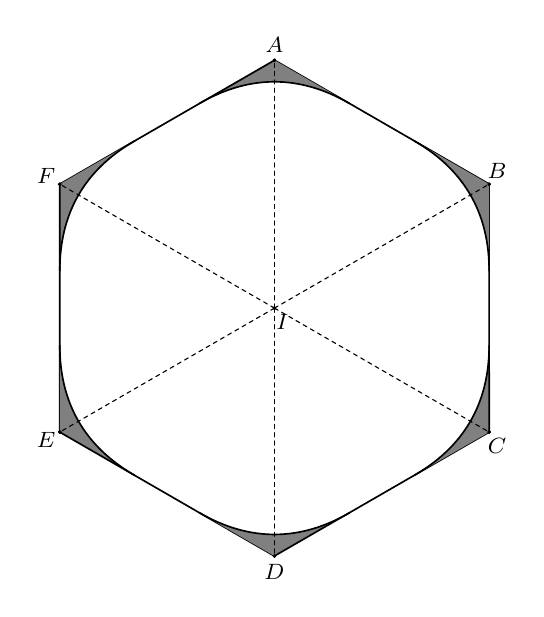
\begin{tikzpicture}[scale=0.025,>=stealth,line join=round,line cap=round,font=\footnotesize]
					\tikzset{declare function={a=126; f (\x)=115-(\x)^2/132; x0=22*sqrt (3);}}
					\path (0,0) coordinate (I)
					\foreach \x/\y in {0/A,1/B,2/C,3/D,4/E,5/F}{
						(I)++({90-\x*60}:a) coordinate (\y)
					};
					\foreach \g in {0,60,...,300}{
						\begin{scope}[rotate=\g]
							\draw [semithick] (0,0)+(30:a)--+(90:a);
							\fill [smooth,samples=100,semithick,gray] plot [domain={-22*sqrt (3)}:{22*sqrt (3)}] (\x,{f (\x)})--(0,a)--cycle;
							\draw [smooth,samples=100,semithick] plot [domain={-22*sqrt (3)}:{22*sqrt (3)}] (\x,{f (\x)});
						\end{scope}
					}
					\foreach \x in {A,B,C,D,E,F}{
						\draw [dash pattern=on 1.5pt off 1.5pt] (I)--(\x);
					}
					\foreach \x/\y in {A/90,B/60,C/-60,D/-90,E/-150,F/150,I/-60}{
						\draw [fill=black] (\x) circle (20pt) ++(\y:8) node {$\x$};
					}
				\end{tikzpicture}
			\end{minipage}\hfill
			\begin{minipage}{.45\linewidth}
				\centering
				\begin{tikzpicture}[scale=0.05,>=stealth,line join=round,line cap=round,font=\footnotesize]
					\tikzset{declare function={a=126; f (\x)=-(\x)^2/132; x0=22*sqrt (3);}}
					\path (0,0) coordinate (O)
					+(0:20) coordinate (O')
					(0,11) coordinate (A)
					(0,-115) coordinate (I)
					($(I)+(30:a)$) coordinate (B)
					($(O)!(B)!(O')$) coordinate (B1)
					($(O)!(B)!(A)$) coordinate (B2)
					(intersection of A--B and O--O') coordinate (T);
					\pic [draw,"$150^\circ$",angle radius=0.2cm,angle eccentricity=1.8] {angle=O'--T--A};
					\fill [smooth,samples=100,semithick,gray] plot [domain=0:{22*sqrt (3)}] (\x,{f (\x)})--(A)--cycle;
					\draw [semithick] (A)--(B);
					\draw [smooth,samples=100,semithick] plot [domain=0:{22*sqrt (3)}] (\x,{f (\x)});
					\draw [dash pattern=on 1.5pt off 1.5pt] (B1)--(B)--(B2);
					\draw [->] (-20,0)--(115,0) node [below,xshift=-3pt] {$x$};
					\draw [->] (0,-63)--(0,30) node [left,yshift=-4pt] {$y$};
					\path (A) node [above right,xshift=-1.7pt] {$11$};
					\foreach \x/\y in {O/-135,A/135,B/-90,T/-90}{
						\draw [fill=black] (\x) circle (20pt) ++(\y:6) node {$\x$};
					}
				\end{tikzpicture}
			\end{minipage}
		\end{center}	
		Gọi lục giác đều là $ABCDEF$ và $I$ là tâm của lục giác đều. \\
		Xét parabol $(P)$ tiếp xúc với hai cạnh $AB$, $AF$. \\
		Chọn hệ trục tọa độ $Oxy$ sao cho gốc tọa độ $O$ trùng với đỉnh của $(P)$, tia $Oy$ chứa điểm $A$ như hình trên (đơn vị trên mỗi trục là cm). \\
		Gọi $S$ là diện tích hình phẳng giới hạn bởi đồ thị $(P)$, đường thẳng $AB$ và trục tung. \\
		Khi đó diện tích phần bị vát đi là $12 \cdot S$. \\
		Theo đề ta có $IA=AB=126$, $IO=115$, $OA=126-115=11$. \\
		Suy ra $A(0;11)$. \\
		Gọi $T$ là giao điểm của $AB$ và $Ox$. \\
		Ta có $\widehat{TAO}=60^\circ$, $\widehat{ATO}=90^\circ-\widehat{TAO}=30^\circ$, $\widehat{ATx}=180^\circ-\widehat{ATO}=150^\circ$. \\
		Do đó đường thẳng $AB$ có hệ số góc $k=\tan 150^\circ=-\dfrac{\sqrt{3}}{3}$. \\
		Phương trình đường thẳng $AB$ là $y=-\dfrac{\sqrt{3}}{3}x+11$. \\
		Vì $(P)$ có đỉnh $O$ nên phương trình có dạng $y=ax^2$. \\
		Xét phương trình $ax^2=-\dfrac{\sqrt{3}}{3}x+11 \Leftrightarrow ax^2+\dfrac{\sqrt{3}}{3}x-11=0 \quad (*)$. \\
		Vì đường thẳng $AB$ tiếp xúc $(P)$ nên $(*)$ có nghiệm kép 
		\[\Leftrightarrow \Delta=0 \Leftrightarrow \left(\dfrac{\sqrt{3}}{3}\right)^2+44a=0 \Leftrightarrow a=-\dfrac{1}{132}.\]
		Nghiệm kép của $(*)$ là $x=-\dfrac{\sqrt{3}}{3 \cdot 2a}=22\sqrt{3}$. \\
		Suy ra $(P) \colon y=-\dfrac{x^2}{132}$ và đường thẳng $AB$ tiếp xúc với $(P)$ tại điểm có hoành độ $x=22\sqrt{3}$. \\
		Ta có \[S=\displaystyle\int\limits_0^{22\sqrt{3}} \left(-\dfrac{\sqrt{3}}{3}x+11+\dfrac{x^2}{132}\right)\mathrm{\,d}x=\dfrac{242\sqrt{3}}{3} \, \left(\text{cm}^2\right).\]
		Diện tích lục giác đều $ABCDEF$ là 
		\[S'=6 \cdot S_{\triangle IAB}=6 \cdot \dfrac{126^2 \cdot \sqrt{3}}{4}=23\,814\sqrt{3} \, \left(\text{cm}^2\right).\]
		Diện tích mặt bàn sau khi đã vát là
		\[S'-12 \cdot S =22\,846\sqrt{3} \, \left(\text{cm}^2\right) \approx 3{,}96 \, \left(\text{m}^2\right).\]
	}
\end{ex}


\begin{ex}%[0D0C2-9]%[TDMZZ19-22]%[Nguyễn Văn Sang]
	Xếp ngẫu nhiên $8$ học sinh lớp $A$, $3$ học sinh lớp $B$, $2$ học sinh lớp $C$ vào $16$ ghế hàng ngang. Gọi $p$ là xác suất để không có hai học sinh nào cùng lớp ngồi ở hai ghế kề nhau. Hãy tính $10^6p$ \textit{(không làm tròn ở các phép tính trung gian và làm tròn kết quả cuối cùng đến hàng đơn vị)}.
	\par
	\shortans[0]{622}
	\loigiai{
		Ta xem $3$ ghế còn trống như $3$ kí hiệu $T$. Khi đó, mỗi cách xếp vị trí chỗ ngồi tương ứng với một dãy gồm $8$ chữ $A$, $3$ chữ $B$, $2$ chữ $C$, và $3$ chữ $T$. Sau khi xác định được vị trí của các lớp, ta mới hoán vị các học sinh cụ thể trong từng lớp.\\
		Vì có $13$ học sinh phân biệt ngồi vào $16$ ghế nên số phần tử của không gian mẫu là:
		$$n(\Omega) = \mathrm{A}_{16}^{13} = \dfrac{16!}{3!}.$$
		Số \textbf{mô hình chữ cái} thỏa mãn điều kiện: không có hai chữ $A$ kề nhau, không có hai chữ $B$ kề nhau, và không có hai chữ $C$ kề nhau.\\
		\textbf{Bước 1: Xếp trước các kí hiệu không phải $A$ ($3B, 2C, 3T$)}
		Số cách sắp xếp $8$ kí hiệu này đứng thành một hàng ngang là:
		$$\dfrac{8!}{3! \cdot 2! \cdot 3!} = 560 \text{ (cách).}$$
		Sau khi xếp xong $8$ kí hiệu này (gọi chung là các khối $X_1, X_2, \dots, X_8$), chúng tạo ra đúng $9$ khe trống xung quanh để chèn các chữ $A$ vào.
		\begin{center}
			\begin{tikzpicture}[scale=1.0, >=stealth]
				% Vẽ 9 vị trí khe trống cho chữ A trước
				\foreach \i in {1,...,9} {
					\draw[dashed, thick, draw=red!80!black, fill=red!5, rounded corners=2pt] (\i*1.3-1.1, -0.6) rectangle ++(0.5,0.5);
					\node[red!80!black, font=\bfseries\small] at (\i*1.3-0.85, -0.3) {$A$};
					\draw[->, dashed, red!80!black, thick] (\i*1.3-0.85, -0.05) -- (\i*1.3-0.85, 0.25);
				}
				
				% Vẽ 8 khối X_i xen kẽ
				\foreach \i in {1,...,8} {
					\draw[thick, draw=teal!80!black, fill=teal!10, rounded corners=3pt] (\i*1.3-0.5, 0.3) rectangle ++(0.7,0.6);
					\node[teal!80!black, font=\bfseries] at (\i*1.3-0.15, 0.6) {$X_{\i}$};
				}
				
				% Chú thích hình vẽ
				\node[anchor=west, teal!80!black, font=\small\itshape] at (0.2, 1.2) {* Dãy $X_1, X_2, \dots, X_8$ là một hoán vị của nhóm $\{3B, 2C, 3T\}$};
				\node[anchor=west, red!80!black, font=\small\itshape] at (0.2, -0.9) {* Có đúng $9$ khe trống để đặt $8$ chữ $A$ vào};
			\end{tikzpicture}
		\end{center}
		Vì có $8$ chữ $A$ nhưng có đến $9$ khe trống, nên để không có hai chữ $A$ nào đứng cạnh nhau thì mỗi khe chỉ được chứa tối đa một chữ $A$. Điều này đồng nghĩa với việc \textbf{ta buộc phải bỏ trống đúng một khe}.\\
		\textbf{Bước 2: Tìm điều kiện hợp lệ cho khe bỏ trống}
		Không phải khe nào cũng được phép bỏ trống. Nếu khe bị bỏ trống nằm giữa hai chữ cái giống nhau (chẳng hạn giữa $B$ và $B$, hoặc giữa $C$ và $C$), thì khi bỏ khe đó đi, hai chữ cái này sẽ lập tức chạm nhau, vi phạm yêu cầu bài toán.
		\begin{center}
			\begin{tikzpicture}[scale=1.0, >=stealth]
				% Khối B bên trái
				\draw[thick, draw=teal!80!black, fill=teal!10, rounded corners=3pt] (0,0) rectangle (0.8,0.7);
				\node[teal!80!black, font=\bfseries\large] at (0.4,0.35) {$B$};
				% Khe trống ở giữa bị bỏ qua
				\draw[dashed, thick, draw=red!80!black, fill=gray!10, rounded corners=2pt] (1.4,0) rectangle (2.4,0.7);
				\node[red!80!black, font=\small\bfseries] at (1.9,0.35) {Trống};
				% Khối B bên phải
				\draw[thick, draw=teal!80!black, fill=teal!10, rounded corners=3pt] (3.0,0) rectangle (3.8,0.7);
				\node[teal!80!black, font=\bfseries\large] at (3.4,0.35) {$B$};
				% Mũi tên chỉ sự va chạm vi phạm
				\draw[<->, thick, red!90!black, bend left=35] (0.4,0.85) to node[above, black, font=\small\sffamily] {Kề nhau $\rightarrow$ Vi phạm!} (3.4,0.85);
			\end{tikzpicture}
		\end{center}
		Do đó, với mỗi cách xếp cố định của $3B, 2C, 3T$, số vị trí đặt khe trống hợp lệ sẽ bằng:
		$$9 - (\text{số cặp } BB \text{ kề nhau}) - (\text{số cặp } CC \text{ kề nhau}).$$
		Từ đây, tổng số mô hình chữ cái hợp lệ trên toàn bộ $560$ cách xếp là:
		$$N = 9 \cdot 560 - S_{BB} - S_{CC}$$
		Trong đó
		\begin{itemize}
			\item $S_{BB}$: Tổng số cặp $BB$ kề nhau xuất hiện trong tất cả các cách xếp.
			\item $S_{CC}$: Tổng số cặp $CC$ kề nhau xuất hiện trong tất cả các cách xếp.
		\end{itemize}
		\textbf{Bước 3: Tính toán các đại lượng thành phần}
		\begin{itemize}
			\item \textbf{Tính $S_{BB}$:} Trong một chuỗi gồm $8$ vị trí, có $7$ cặp vị trí liên tiếp nhau. Nếu ta buộc một cặp vị trí liên tiếp là $BB$ (xem như $1$ khối cố định), thì $6$ vị trí còn lại sẽ chứa các kí hiệu $\{1B, 2C, 3T\}$. Số cách hoán vị chúng là $\dfrac{6!}{1! \cdot 2! \cdot 3!} = 60$. Vì có $7$ vị trí đặt khối $BB$ nên:
			$$S_{BB} = 7 \cdot 60 = 420.$$
			\item \textbf{Tính $S_{CC}$:} Tương tự, buộc một cặp vị trí liên tiếp là $CC$ (xem như $1$ khối cố định). Khi đó $6$ vị trí còn lại sẽ chứa các kí hiệu $\{3B, 3T\}$. Số cách hoán vị chúng là $\dfrac{6!}{3! \cdot 3!} = 20$. Do đó
			$$S_{CC} = 7 \cdot 20 = 140.$$
		\end{itemize}
		Suy ra tổng số mô hình sắp xếp chữ cái hợp lệ là
		$$N = 9 \cdot 560 - 420 - 140 = 4480 \text{ (mô hình)}.$$
		\textbf{Bước 4: Tính xác suất và kết luận}
		Với mỗi mô hình chữ cái định sẵn, ta có
		\begin{itemize}
			\item $8!$ cách xếp các học sinh cụ thể của lớp $A$.
			\item $3!$ cách xếp các học sinh cụ thể của lớp $B$.
			\item $2!$ cách xếp các học sinh cụ thể của lớp $C$.
		\end{itemize}
		Số kết quả thuận lợi cho biến cố là
		$$n(A) = 4480 \cdot 8! \cdot 3! \cdot 2!.$$
		Xác suất cần tìm bằng
		$$p = \dfrac{n(A)}{n(\Omega)} = \dfrac{4480 \cdot 8! \cdot 3! \cdot 2!}{\dfrac{16!}{3!}} = \dfrac{4}{6435}.$$
		Giá trị đại lượng đề bài yêu cầu
		$$10^6p = 10^6 \cdot \dfrac{4}{6435} \approx 622.$$
	}
\end{ex}